\documentclass[a0paper,smallertitle]{HYposter}

\usepackage[utf8]{inputenc}
\usepackage[english]{babel}
\usepackage{amsmath,amsthm, amssymb}
\usepackage{algorithmicx}
\usepackage{algorithm}

\newcommand{\url}[1]{\texttt{#1}}

%Macros
\DeclareMathOperator*{\argmin}{arg\,min}
\DeclareMathOperator{\Corr}{Corr}


\title{\hspace{20mm}Parallel \texttt{stable k-means}}
\author{Emin Arakelian \hspace{5mm}  \url{emin@berkeley.edu}  \\
Fadi Kfoury \hspace{5mm}  \url{fadi.kfoury@berkeley.edu}  \\
Jason Poulos \hspace{5mm}  \url{poulos@berkeley.edu}  }
\affiliation{}
\thanks{}


\begin{document}

\section*{Introduction} \label{section:Intro}

$k$-means is a popular unsupervised learning algorithm for finding clusters and cluster centers in data. The goal is to choose $k$ cluster centers to minimize the total squared distance between each data point and its closest center. One method to determine the optimal number of clusters is stability. Assessing stability requires multiple runs of $k$-means, which will make it computationally very expensive.


\section*{Serial \texttt{stable k-means}} \label{section:stable}
Ben-Hur et al.\cite{ben2001} propose an algorithm for any clustering mechanism that will assess the stability of the points and thus let us infer the optimal number of clusters. %The algorithm begins with subsampling the data twice with a ration more than half. It is believed that the general structure of the dataset is captured when subsampling with a ration bigger than a half. Then, for a given number of clusters, the two subsamples are clustered. The points in the intersection of the two subsamples are analyzed to see how many of them are clustered together in the same cluster in both subsamples. Then, depending on the number of the points clustered together in the intersection of both of the subsamples, a similarity score is calculated. We will use the correlation score for our application.
%
Let labeling $\mathcal{L}$ be a partition of $X$ into $k$ subsets $S_1, S_2, ... , S_k$. In that case the correlation score between the clustering of intersection of two subsamples is given by: 

\[
\Corr(\mathcal{L}_1, \mathcal{L}_2) = \frac{\langle \mathcal{L}_1, \mathcal{L}_2 \rangle}{\sqrt{\langle \mathcal{L}_1,\mathcal{L}_1\rangle \langle \mathcal{L}_2,\mathcal{L}_2\rangle}}
\] The algorithm for \texttt{stable k-means} is displayed in Algorithm \ref{alg:stability}.

\begin{algorithm}[H] 
\textbf{Input}: $X$ \{a dataset\}, $k_{max}$ \{maximum number of
clusters\}, num\_subsamples \{number of subsamples\} 

\textbf{Output}: $S(i,k)$ \{list of similarities for each $k$ and
each pair of sub-samples\}

\textbf{Require}: A clustering algorithm: cluster$(X,k)$ ; a similarity
measure between labels: $s(\mathcal{L}_1,\mathcal{L}_2)$

1: $f = 0.7$ 

2: for $k=2$ to $k_{max}$ \textbf{do} 

3: for $i=1$ to $num_subsamples$ \textbf{do} 

4: $sub_1 = $subsamp$(X, f)$ \{a sub-sample with a fraction of $f$
the data\} 

5: $sub_2 = $subsamp$(X, f)$ 

6: $\mathcal{L}_1=$cluster$(sub_1, k)$ 

7: $\mathcal{L}_2=$cluster$(sub_2, k)$ 

8: Intersect $= sub_1 \cap sub_2$

9: $S(i, k) = s(\mathcal{L}_1(Intersect), \mathcal{L}_2(Intersect))$
\{Compute the similarity on the points common to both subsamples\} 

10: \textbf{end for }

11: \textbf{end for}

\caption{\label{alg:stability}}
\end{algorithm}

%Given this algorithm, for each $k$, a distribution of scores will be attained. The distribution with the highest score and least variance is the best; distributions that are unimodal are also highly preferred. These criteria means that the consistently intersection points were clustered together and thus that certain formation of clusters was stable.

%\section*{Parallelization} \label{parallel}

\section*{Threading and the GIL}

%Python utilizes a multithreading module letting the user use multiple
%threads. Python threads are real system threads, i.e. Posix threads
%or Windows threads and are fully operated by the host operating system.
%The caveat however is that for CPU-bound functions, the threaded version
%will perform worse than the serial version. The reason behind that
%is that parallel execution is forbidden in Python and there is a GIL,
%Global Interpreter Lock, that ensures only one thread is ran at a
%time in the interpreter which simplifies many of the low level tasks
%like memory management and call out to C extensions. 

With the existence
of GIL we get a cooperative multitasking as shown in Figure \ref{fig:Cooperative-multitasking-with}.
When a thread is running it is holding the GIL and the GIL is released
upon I/O commands such as read, write, send, receive etc. Thus the
merit of multithreading will be apparent when the functions are I/O
bound. 

\begin{figure}[H] 
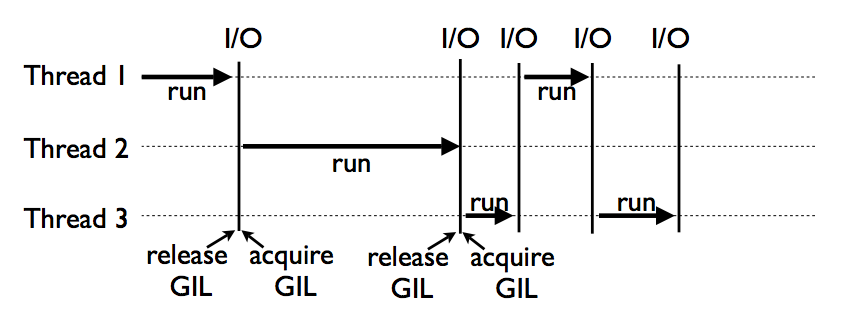
\includegraphics[width=\columnwidth]{/Users/jason/Dropbox/github/parallel_kmeans/report/figure/threads_IO.png}
\caption{Cooperative multitasking with GIL} \label{fig:Cooperative-multitasking-with}
\end{figure}

CPU-bound threads that never perform I/O are handled differently where
there are special check for every 100 ``ticks'', see Figure \ref{fig:No-I/O-function}.
%These ticks should not be confused with the clock ticks. These ticks
%are roughly equivalent to one interpreter instruction. The check is
%as follows, the current thread will reset the tick counter, reset
%the signal handler if it is the main thread, release the GIL and reacquire
%it.

\begin{figure}[H] 
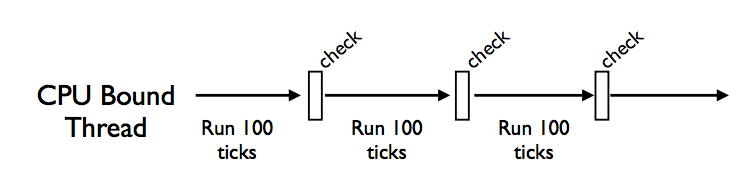
\includegraphics[width=\columnwidth]{/Users/jason/Dropbox/github/parallel_kmeans/report/figure/threads_check.png}
\caption{No I/O function checks}
\label{fig:No-I/O-function}
\end{figure}

In thread switching on a single core two cases can happen. %Assume
%we have two threads, with the first thread running. If at some point
%the first thread has an I/O instruction, it will release the GIL and
%the second thread will acquire it. However, if the first thread has
%no I/O instructions, then the GIL release will happen on the check.
%In which case the lock is free and two threads are ready to run. Here
%the priority will be handled by the OS, and the next thread may or
%may not be thread 2, however experimental result has shown that this
%thread switching happens rarely, and there would be thousands of checks
%before thread two will run. A more interesting problem arises when
%multiple cores have runnable threads. Here the threads get scheduled
%simultaneously on multiple cores and thus they will battle over the
%GIL. This happens because when thread one releases the GIL and signals
%universally, thread two takes some time to wake up to acquire the
%lock, by which time thread one has acquired the lock and thread two,
%failing at it's endeavors decides to sleep again. 
An illustration is provided in Figure \ref{fig:GIL-wars-on}.

\begin{figure}[H] 
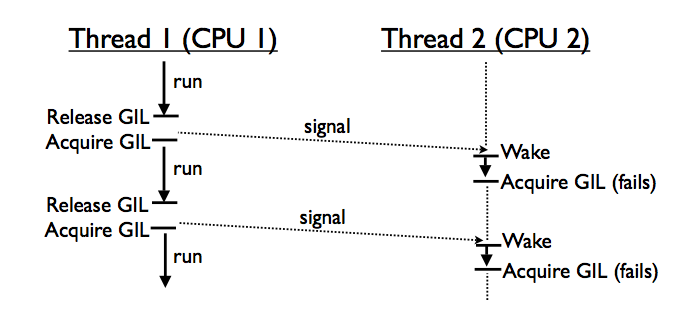
\includegraphics[width=\columnwidth]{/Users/jason/Dropbox/github/parallel_kmeans/report/figure/threads_multicore.png}
\caption{GIL wars on multicored threads}
\label{fig:GIL-wars-on}
\end{figure}

%To remedy this problem, in Python 3 is a new GIL implementation that
%allows thread two to signal a timeout in which case thread one will
%drop the lock after its current instruction and thread two can take
%over. This seems to address the problem a little, but still there
%are starvation scenarios where the most deserving threads do not get
%to run first due to scheduling. A suggested work around for this is
%to separate CPU-bound, low priority threads and I/O, high priority
%threads. 

\section*{Multiprocessing}

A good alternative to multithreading is multiprocessing which came
about around Python 2.6. The syntax is exactly the same as multithreading
but here python uses processes instead of threads and thus eliminating
shared anything. Here we will have multiple instances of the interpreter
running each having their own GIL and the way they communicate is
message passing. The messages are being passed using ``pickle''-ing.
The pickle module in Python can serialize and deserialize python objects
into byte-streams. Since we are using message passing here, we can
deploy our code on multiple machines as well. 

\section*{Experiments} \label{implementation}

We will run our algorithm and compare its results on a toy dataset
of 500 samples and 2 features. The dataset is plotted in Figure \ref{fig:Dataset-that-will}. The dataset is obviously split into 5 clusters at most. Running the
algorithm on this dataset will yield the following similarity scoring
distribution (Figure \ref{fig:Histograms-of-Similarity}).

\begin{figure}[H] 
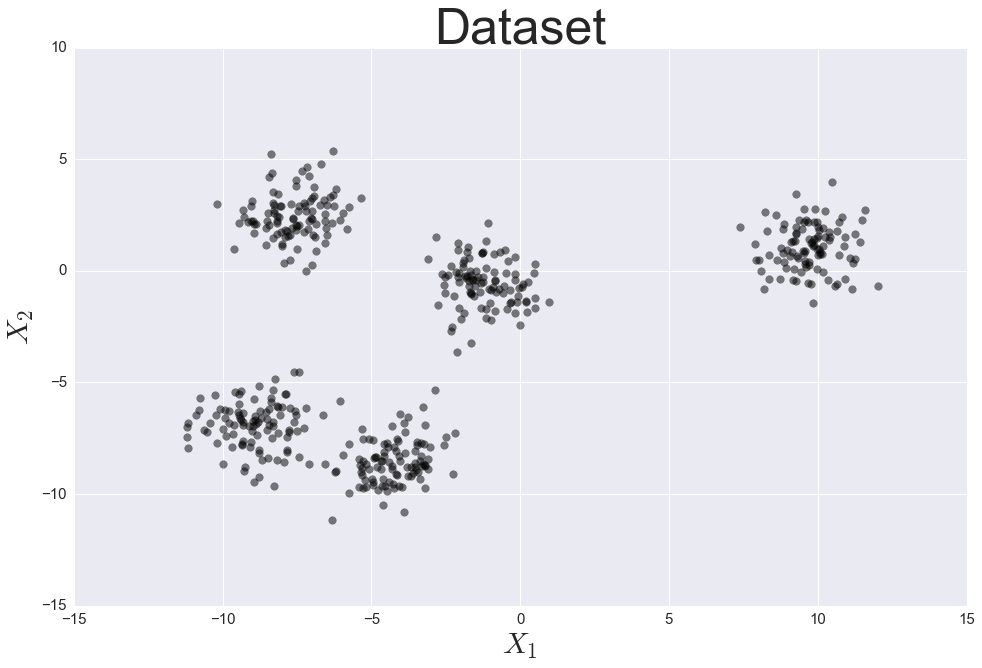
\includegraphics[width=\columnwidth]{/Users/jason/Dropbox/github/parallel_kmeans/report/figure/dataset.png}
\caption{\label{fig:Dataset-that-will}Dataset that will be used to assess
\texttt{stable k-means}}
\end{figure}

\begin{figure}[H] 
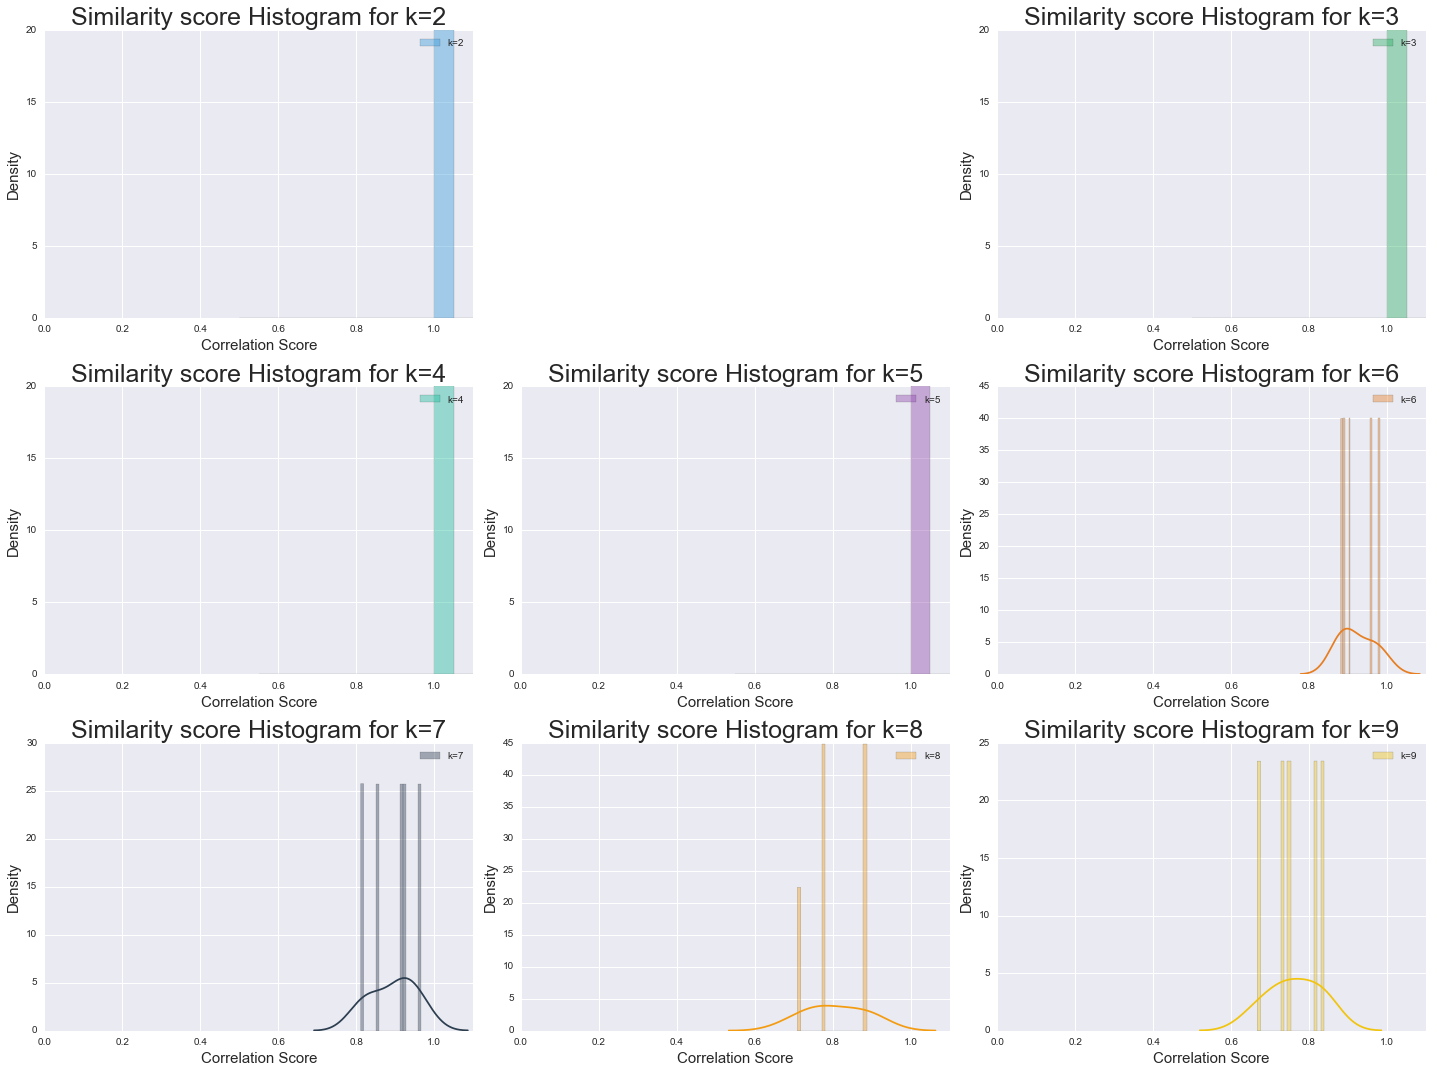
\includegraphics[width=\columnwidth]{/Users/jason/Dropbox/github/parallel_kmeans/report/figure/histogram.png}
\caption{\label{fig:Histograms-of-Similarity}Histograms of Similarity scores
for different ks.}
\end{figure}

%Figure \ref{fig:Serial-Run-Time} shows the baseline serial run time; Figure \ref{fig:Strong-and-Weak} shows the strong and weak scaling of the multithread and multiprocess algorithms; Figure \ref{fig:Speed-up-Comparison} below shows a comparison of the run time on the serial, concurrent (multithread) and parallel (multiprocess) code.

\begin{figure}[H] 
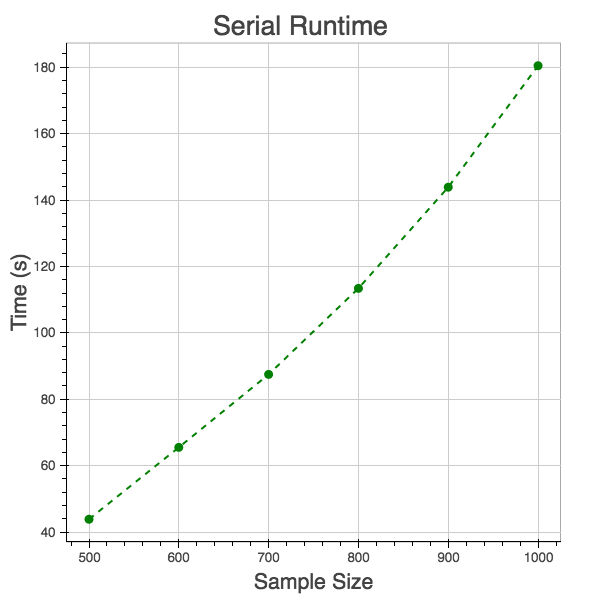
\includegraphics[width=\columnwidth]{/Users/jason/Dropbox/github/parallel_kmeans/report/figure/serial.png}
\caption{\label{fig:Serial-Run-Time}Serial Run Time}
\end{figure}


\begin{figure}[H] 
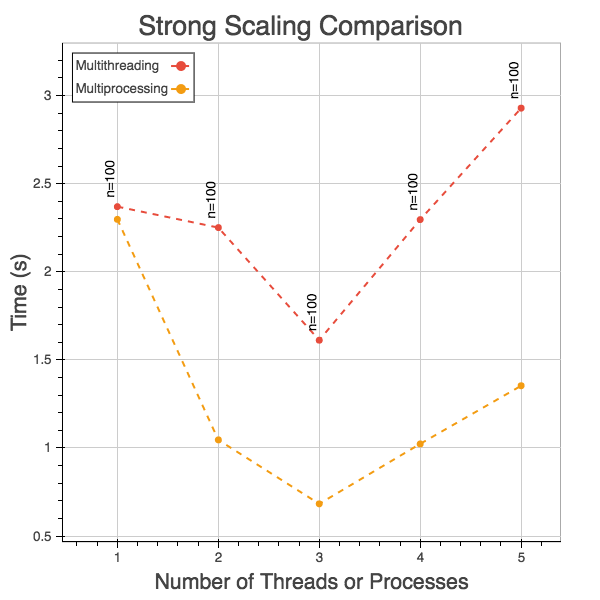
\includegraphics[width=\columnwidth]{/Users/jason/Dropbox/github/parallel_kmeans/report/figure/mt_mp_ss_comp.png} 
\caption{\label{fig:Strong-and-Weak}Strong and Weak Scaling Comparison for
Multithreading and Multiprocessing}
\end{figure}

\begin{figure}[H] 
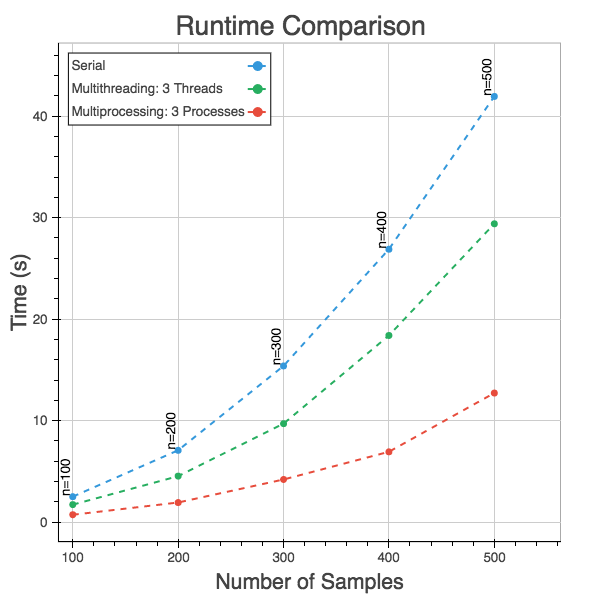
\includegraphics[width=\columnwidth]{/Users/jason/Dropbox/github/parallel_kmeans/report/figure/runtime_comparison.png}
\caption{\label{fig:Speed-up-Comparison}Speed up Comparison}
\end{figure}

%\section*{Challenges and Future Directions} \label{challenges}

%\section*{Conclusion} \label{conclusion}

% References
\begin{thebibliography}{5}
\bibitem{ben2001} Ben-Hur, Asa and Elisseeff, Andre and Guyon, Isabelle. "A stability based method for discovering structure in clustered data." \emph{Pacific symposium on biocomputing} 7 (2001): 6-17.
\end{thebibliography}

\end{document}
